% *** DOCUMENT CLASS ***
\documentclass{llncs}

% *** MATH ***
\usepackage{amsmath,amssymb,amsfonts}
\usepackage{theorem}
\usepackage{times,mathptm}

% *** ALIGNMENT PACKAGES ***
%
\usepackage{array}
\usepackage{tabularx,ragged2e,booktabs}

% *** SUBFIGURE PACKAGES ***
%\usepackage[font={small}]{caption, subfig}
\usepackage[font=footnotesize]{caption, subfig}

% *** FLOAT PACKAGES ***
%
\usepackage{stfloats}

% *** CITATION PACKAGES ***
\usepackage{cite}

% *** GRAPHICS RELATED PACKAGES ***
\usepackage[dvips]{graphicx}
\graphicspath{{figures/}}
\DeclareGraphicsExtensions{.eps}

% *** MISC PACKAGES ***
%
%%% additional font formatting capability
\usepackage{ulem}
\newcommand{\msout}[1]{\text{\sout{\ensuremath{#1}}}}
%
%%% PACKAGE FOR USING THE MULTI-LINE COMMENT
\usepackage{verbatim}
%
%%% COLORS
\usepackage{color}


% *** SETTINGS AND MACROS ***
%% Package to linebreak URLs in a sane manner.
\usepackage{url}
\makeatletter
\def\url@smallurlstyle{%
  \@ifundefined{selectfont}{\def\UrlFont{\sf}}{\def\UrlFont{\small\ttfamily}}}
\makeatother
\urlstyle{smallurl}
\makeatletter
\def\url@tinyurlstyle{%
  \@ifundefined{selectfont}{\def\UrlFont{\sf}}{\def\UrlFont{\scriptsize\ttfamily}}}
\makeatother
\renewcommand{\UrlFont}{\scriptsize}
%
%% Make URLs clickable
\usepackage[colorlinks, bookmarks=false]{hyperref}
%\usepackage{hyperref}
\usepackage{breakurl}
\hypersetup{ colorlinks=false, citecolor=black,
    filecolor=black, linkcolor=black, urlcolor=black
}

% *** FIXME NOTES ***
%
\usepackage[margin=false,inline=false,marginclue,draft]{fixme}
% REMOVE draft to disable fixme notes
%\usepackage[margin,inline,marginclue]{fixme}
%
\makeatletter
\renewcommand*\FXLayoutInline[3]{%
  {\@fxuseface{inline}\ignorespaces[#3 \fxnotename{#1}: #2]}}
\makeatother

\hyphenation{SAXSequitur}

%
% paper title
% can use linebreaks \\ within to get better formatting as desired
\title{SAXSequitur GUI: a tool for grammar-based\\ patterns discovery in time series}

\begin{document} 
\author{Pavel Senin\inst{1} \and Jessica Lin \inst{2} \and Xing Wang \inst{2} \and Rasaq Otunba \inst{2} \and \\ Tim Oates\inst{3} \and Manfred Lerner \inst{4}}
%\and \\Arnold P. Boedihardjo\inst{3} \and Tim Oates\inst{4} \and \\ Crystal Chen\inst{3} \and Susan Frankenstein\inst{3} \and Sunil %Gandhi\inst{4}}

\institute{University of Hawaii, Manoa,
 Dept. of Computer Science, \\
 \email{senin@hawaii.edu}
 \and George Mason University,
 Dept. of Computer Science, \\
 \email{\{jessica, xwang24, rotunba\} @gmu.edu}
 %\and
 %U.S. Army Corps of Engineers,
 %Engineer Research and  Development Center,
 %\email{\{arnold.p.boedihardjo, crystal.chen, susan.frankenstein\}@usace.army.mil}
 \and
 University of Maryland, Baltimore County,
 Dept. of Computer Science,
 \email{oates@cs.umbc.edu}
 \and SAP Germany,
 \email{manfred.lerner@sap.com}
}
\maketitle

\begin{abstract}
The problem of recurrent and anomalous patterns discovery in time series has received a lot of attention from researchers in the past decade. Addressing the common limitation of existing techniques, which require a pattern length to be known in advance, we recently proposed grammar-based algorithms for efficient discovery of co-existing variable length recurrent and anomalous patterns (i.e. motifs and discords). In this demo paper we present SAXSequitur GUI - an interactive tool that implements our algorithms for grammar-driven time series patterns mining and visualization.
\end{abstract}

%\keywords{time series mining, anomaly discovery, frequent patterns discovery}

%\begin{small}
%\section{Paper requirements}
%\textit{A demonstration submission must be up to 4 pages long. It must provide adequate information on the system’s components and the way the system is operated. Figures, screenshots and interactive demonstration plans may be included if necessary. The authors must further provide a URL that points to a preview of the demonstration which can be seen as a companion webpage including more material, a detailed documentation and if possible the tool itself.}

%\textit{Submitters should keep in mind that the description of a demo has inherently different content than a research paper submitted to the main conference. A successful demonstration paper provides satisfactory answers the following questions:}
%\begin{enumerate}
% \item What makes the presented piece of software unique and special?
% \item What are the innovative aspects or in what way/area does it represent the state of the art?
% \item For whom is it most interesting/useful – for an ML/DM researcher, for a graduate or undergraduate student in these areas, for a practitioner?
% \item If there are similar/related pieces of software, what are the advantages and disadvantages of the presented one?
%\end{enumerate}
%\end{small}

\section{Introduction}
The ability to efficiently detect recurrent and anomalous patterns in time series allows to explore, to summarize, and to compress the data. In addition, such information is crucial in a variety of application domains where these patterns convey critical and actionable information, such as in health care, equipment safety, and security. Finally, these patterns are often used as input features for machine learning techniques, such as association rules mining. % \cite{association_rules}

Previously, we defined time series motifs \cite{lin_motifs}, which are recurrent patterns, and time series discords \cite{hot_sax}, which are anomalies, and proposed an efficient \textit{exact} solutions for their discovery based on Symbolic Aggregate Approximation (SAX) \cite{sax}. While our techniques perform at the level of current state of the art \cite{chan_anomaly}, similarly to many other approaches for time series patterns discovery, they require the length of a potential motif or discord to be specified as an input, which is unreasonable to expect to be known in advance for many real-world problems.

Addressing the aforementioned limitation, we recently proposed an alternative solutions for variable-length motifs \cite{grammarviz} and discords discovery [?] based on SAX discretization and Sequitur grammar inference algorithm \cite{sequitur}. As we has shown, when configured only by discretization parameters and given a ``seeding'' sliding window length, our algorithms are capable to efficiently discover \textit{co-existing variable-length approximate motifs and discords} without any prior knowledge about their length, shape, or minimal occurrence frequency.
%Note, that it has been recently shown that in many applications, approximate solutions might be sufficient or even preferable due to efficiency \cite{grammarviz}. 

\section{SAXSequitur GUI - an interactive tool to time series mining}
In this paper we present a Graphical User Interface (GUI) application that is a prototype implementing our grammar-based patterns discovery algorithms in Java, whose source code is available at \cite{jmotif}. It has a simple interface allowing the user to load the data, to discretize it, to infer a context-free grammar, and to visualize time-series subsequences corresponding to grammar rules. In addition, since grammar rules tend to be numerous and overlapping (Fig.\ref{fig1}), our tool provides an efficient heuristic for their pruning. Finally, it implements our recently proposed grammar-driven time series anomaly discovery algorithms based on the grammar rules density and distance computation [?].

\begin{figure}[t]
   \vspace{-0.8cm}
   \centering
   \includegraphics[width=120mm]{Figure1_TEK16_R95.eps}
   \caption{An example of recurrent grammar rule (i.e. \textbf{\textit{motif}}) discovered in Space Shuttle Marotta Valve (TEK) dataset \cite{hot_sax}. Rule-corresponding subsequences highlight a normal de-energizing phase found in all valve cycles. (\textit{note that two pairs of rule occurrences overlap})}
   \label{fig1}
   \vspace{-0.4cm}
\end{figure}

As time series often used as a proxy representing a large variety of real-life phenomena in a wide range of domains, SAXSequitur GUI targets diverse audiences among which are researchers, engineers, medical specialists, and safety and security personnel. Our tool provides interactive parameters tuning and patterns visualization, which are \textit{essential capabilities} aiding in discretization parameters selection.

SAXSequitur GUI implements Model-View-Controller (MVC) software architectural pattern, therefore, due to its modular structure, it can be easily modified into a client-server web-application or a web-service providing a federated access to data and computational resources in industrial settings. 

Further in this section we briefly discuss the grammar-driven time series mining paradigm and data processing details by implemented algorithms which enables efficient variable-length approximate patterns discovery in time series.

\subsection{Dimensionality reduction and discretization with SAX}
Time series are continuous data while grammar induction algorithms are designed for discrete values. We rely on SAX \cite{sax} for time series discretization. For time series $T$ of length $m$, SAX obtains its lower-dimensional representation by \textit{z}-normalizing and dividing it into $w$ equal-sized segments at first. Next, for each segment, the algorithm computes a mean value and maps it to a symbol according to a pre-defined set of breakpoints dividing the data distribution space into $\alpha$ equiprobable regions, where $\alpha$ is the alphabet size specified by the user. 

Note, that dimensionality reduction is embedded into the SAX discretization process as $w$ is almost always much smaller than the original sequence length $m$. While this is a desirable feature for exploring global patterns, in the case where we are interested in a localized phenomena, the high compression ratio ($m/w$) significantly affects the technique's performance. Thus, for local patterns discovery, and specifically for motifs and discords discovery, SAX is often applied to a set of subsequences that represent local features -- the technique called subsequence discretization \cite{lin_motifs} -- where subsequences extraction is implemented via sliding window. Note that our tool implements the both options: global and local discretization as shown at Fig.\ref{fig1} (``SAX parameters'' panel). 

The same panel allows the user to specify other discretization parameters and to toggle the numerosity reduction strategy, that is an essential part of our technique that not only allows to mitigate the trivial and degenerate patterns discovery, but enables a unique feature -- the ability to discover variable-length patterns as we discuss in [?]. 

\begin{figure}[t]
   \vspace{-0.8cm}
   \centering
   \includegraphics[width=120mm]{Figure2_TEK16_R92.eps}
   \caption{An example of anomalous grammar rule discovered in TEK dataset. Corresponding to the rule subsequence highlights an abnormal energizing phase in a valve cycle.}
   \label{fig2}
   \vspace{-0.4cm}
\end{figure}

\subsection{Context free grammar induction with Sequitur}
For grammar inference, we rely on Sequitur - a linear time and space algorithm that derives a context-free grammar from a string incrementally \cite{sequitur}. By identifying recurrent subsequences in the input string, the algorithm builds a compact context-free grammar reflecting the input string specificity. 
%Although simple in design, Sequitur has been shown to be competitive with state of the art compression algorithms even for very large strings. 

\section{Exploiting context-free grammar for patterns discovery}
Rules of a context free grammar are hierarchically organized. By the analysis of a grammar's hierarchy, SAXSequitur identifies rules which are frequently used and those which are rarely used by other grammar's rules and specifically by the root rule \textit{R0} that represents a full time series span. Intuitively, as each of the rules represents a discretized subsequence of the input time series, frequently used rules are likely to correspond to recurrent subsequences while rules which are rarely used, likely to correspond to rare subsequences.\\
\textit{\textbf{Motif discovery}}. SAXSequitur GUI allows to highlight locations of all subsequences corresponding to the selected rule and to superimpose all subsequences at the same plot enabling visual evaluation of selected parameters performance and recurrent patterns discovery by following our intuition (Fig.\ref{fig1}).\\
{\parindent0pt
\textit{\textbf{Discord discovery}}. Similarly, the user is able to visually evaluate the selected rule potential to be an anomaly, moreover, implemented in our tool algorithms provide additional evidence for examined subsequences -- visualization of their coverage grammar rules (Fig.\ref{fig3}) and the exact distance to the nearest neighbor (Fig.\ref{fig2}).
}\\
{\parindent0pt
\textit{\textbf{Periodicity discovery}}.
In [?] we introduced a notion of the approximate period. \\ SAXSequitur GUI allows to visualize intra-motif subsequences thus enabling an approximate periodicity discovery (Fig.\ref{fig3}).}

\begin{figure}[t]
   \vspace{-0.8cm}
   \centering
   \includegraphics[width=120mm]{TEK16_DataDisplayScreens.eps}
   \caption{Examples of ``Data display'' panel showing from top to bottom: a rules density plot used for highly efficient approximate anomaly discovery, a periodicity plot highlighting putative periodic subsequences (a normal valve de-energizing periods), and the rules length histogram providing a descriptive statistics.}
   \label{fig3}
   \vspace{-0.4cm}
\end{figure}
\enlargethispage{1.5cm}

\begin{thebibliography}{4}

%1
%\bibitem {association_rules}
%Agrawal, R., Imieliński, T., Swami, A.:
%Mining association rules between sets of items in large databases. 
%In Proc. of ACM SIGMOD Intl. Conference on Management of data, (1993)

%2
\bibitem {lin_motifs}
Lin, J., Keogh, E., Patel, P., and Lonardi, S.: 
Finding Motifs in Time Series., The 2nd Workshop on Temporal Data Mining, the 8th ACM Int'l Conference on KDD. 53--68, (2002)

%3
\bibitem {hot_sax}
Keogh, E., Lin, J., Fu, A.:
HOT SAX: Efficiently Finding the Most Unusual Time Series Subsequence. 
In Proc. ICDM. 226--233, (2005)

%4
\bibitem {sax}
Patel, P., Keogh, E., Lin, J., Lonardi, S.:
Mining Motifs in Massive Time Series Databases. 
In Proc. ICDM, (2002)

%5
\bibitem{chan_anomaly} 
Chandola, V., Cheboli, D., and Kumar, V.:
Detecting Anomalies in a Time Series Database.
CS Technical Report 09--004, (2009)

%6
\bibitem{grammarviz}
Li, Y., Lin, J., and Oates, T.: 
Visualizing variable-length time series motifs. 
In Proc. of the 2012 SIAM International Conference on Data Mining, 895-906, (2012)

%7
\bibitem {sequitur}
Nevill-Manning, C. and Witten, I.:
Identifying Hierarchical Structure in Sequences: A linear-time algorithm. 
Journal of Artificial Intelligence Research, 7, 67-82, (1997)

%17
\bibitem {jmotif}
Paper authors. Supporting webpage:
\url{https://code.google.com/p/jmotif/}

% %%%%%%%%%%%%%%%%%%%%%%%%%%%%%%%%
% not used
%

\begin{comment}

%7
\bibitem {outliers_survey}
Gupta, M., Gao, J., Aggarwal, C.C., Han, J.:
Outlier Detection for Temporal Data: A Survey.
IEEE Trans. on Knowledge and Data Engineering, 25, 1, (2013)

%3
\bibitem{hawkins} 
Hawkins, D. M.: 
Identification of Outliers. Chapman and Hall, (1980)

%8
\bibitem{hashing} 
Wei, L., Keogh, E., Xi, X.: 
SAXually explicit images: Finding unusual shapes.
In Proc. of the 6th International Conference on Data Mining, 711--720, (2006)

%9
\bibitem{haar_1} 
Fu, A., Leung, O., Keogh, E., Lin, J.:
Finding Time Series Discords based on Haar Transform.
In Proc. of the 2nd Intl. Conf. on Advanced Data Mining and Applications. 31--41 (2006)

%10
\bibitem{haar_2} 
Bu, Y., Leung, O., Fu, A., Keogh, E., Pei, J., Meshkin, S.:
WAT: Finding Top-K Discords in Time Series Database.
In Proc. of the 7 th SIAM Intl. Conf. on Data Mining. 449--454 (2007)

%11
\bibitem{disk} 
Yankov, D., Keogh, E., Rebbapragada, U.:
Disk aware discord discovery: finding unusual time series in terabyte sized data sets.
Knowledge and Information Systems, 241--262 (2008).

%12
\bibitem{viztree}
J. Lin, E. Keogh, S. Lonardi, J. P. Lankford, and D. M. Nystrom.:
Visually mining and monitoring massive time series. 
In Proc. 10th ACM SIGKDD Intl. Conf. on Knowledge Discovery and Data Mining, 460-469 (2004). 

%13
\bibitem{ano_pattern} Chen, X., Zhan, Y.:
Multi-scale Anomaly Detection Algorithm based on Infrequent Pattern of Time Series.
Journal of Computational and Applied Mathematics. 227--237 (2008)

%14
\bibitem{bitmaps} Wei, L., Kumar, N., Lolla, V., Keogh, E., Lonardi, S., Ratanamahatana, C.:
Assumption-free Anomaly Detection in Time Series.
In Proc. of the 17th Intl. Conf. on Scientific and Statistical Database Management (SSDBM), 237--240, (2005)

\enlargethispage{\baselineskip}
%16
\bibitem {physionet}
A. L. Goldberger, L. A. Amaral, L. Glass, J. M. Hausdorff, P. Ivanov, R. Mark, J.  Mietus, G. Moody, C. Peng, and H. Stanley. 
PhysioBank, PhysioToolkit, and PhysioNet: components of a new research resource for complex physiologic signals. 
Circulation, 101(23), (2000)

%not used
\bibitem{sax_tries} 
\fxnote[inline]{not used} 
Lin, J., Keogh, E., Fu, A., Herle, H. Van.:
Approximations to Magic: Finding Unusual Medical Time Series.
In Proc. of the 18 th IEEE Symposium on Computer-Based Medical Systems (CBMS). 329--334 (2005)

%not used
\bibitem {exp_sax}
\fxnote[inline]{not used} 
Lin, J., Keogh, E., Wei, L., Lonardi, S.:
Experiencing SAX: a novel symbolic representation of time series.
Data Min. Knowl. Discov., 107--144 (2007)

%not used
\bibitem {keogh_linear}
\fxnote[inline]{not used} 
Keogh, E., Lonardi, S., Chiu, B. Y.-c.:
Finding Surprising Patterns in a Time Series Database in Linear Time and Space,
in Proc. SIGKDD (2002)

%not used
\bibitem {motion_motif_graphs}
\fxnote[inline]{not used} 
P. Beaudoin, M. van de Panne, P. Poulin and S. Coros. 
(2008) Motion-Motif Graphs. In Proc. of the Symposium on Computer Animation.
\end{comment}
\end{thebibliography}

% \section*{Appendix: Springer-Author Discount}
% 
% LNCS authors are entitled to a 33.3\% discount off all Springer
% publications. Before placing an order, the author should send an email, 
% giving full details of his or her Springer publication,
% to \url{orders-HD-individuals@springer.com} to obtain a so-called token. This token is a
% number, which must be entered when placing an order via the Internet, in
% order to obtain the discount.
% 
% \section{Checklist of Items to be Sent to Volume Editors}
% Here is a checklist of everything the volume editor requires from you:
% 
% 
% \begin{itemize}
% \settowidth{\leftmargin}{{\Large$\square$}}\advance\leftmargin\labelsep
% \itemsep8pt\relax
% \renewcommand\labelitemi{{\lower1.5pt\hbox{\Large$\square$}}}
% 
% \item The final \LaTeX{} source files
% \item A final PDF file
% \item A copyright form, signed by one author on behalf of all of the
% authors of the paper.
% \item A readme giving the name and email address of the
% corresponding author.
% \end{itemize}
\end{document}
